% This is samplepaper.tex, a sample chapter demonstrating the
% LLNCS macro package for Springer Computer Science proceedings;
% Version 2.21 of 2022/01/12
%
\documentclass[runningheads]{llncs}
%
\usepackage[T1]{fontenc}
% T1 fonts will be used to generate the final print and online PDFs,
% so please use T1 fonts in your manuscript whenever possible.
% Other font encondings may result in incorrect characters.
%
\usepackage{graphicx}
% Used for displaying a sample figure. If possible, figure files should
% be included in EPS format.
%
% If you use the hyperref package, please uncomment the following two lines
% to display URLs in blue roman font according to Springer's eBook style:
%\usepackage{color}
%\renewcommand\UrlFont{\color{blue}\rmfamily}
%\urlstyle{rm}
%
\begin{document}
%
\title{Contribution Title}
%
%\titlerunning{Abbreviated paper title}
% If the paper title is too long for the running head, you can set
% an abbreviated paper title here
%
\author{First Author}
%
\authorrunning{F. Author et al.}
% First names are abbreviated in the running head.
% If there are more than two authors, 'et al.' is used.
%
\institute{Technical University of Denmark}


\maketitle              % typeset the header of the contribution
%
\begin{abstract}

The abstract should briefly summarize the contents of the paper in
150--250 words.

\begin{itemize}
    \item I use this as a reference - https://www.ias.informatik.tu-darmstadt.de/HowTo/WritingAnEffectiveAbstract
    \item Should be effectively very concise, no filler words, simple sentences
    \item Context $\rightarrow$ Problem $\rightarrow$ Methods $\rightarrow$ Key Findings
\end{itemize}

\keywords{First keyword  \and Second keyword \and Another keyword.}
\end{abstract}
%
%
%
\section{Introduction}

\begin{itemize}
    \item Use the 'inverted triangle' or 'funnel' approach - https://www.thegoldenthread.nl/research-paper-strategy-the-introduction/
    \item Big picture problem, motivation $\rightarrow$ fairness $\rightarrow$ medical imaging $\rightarrow$ medical segmentation.
    \item Highlight our arguments (e.g., fairness in segmentation is much harder/complex than segmentation due to X, Y, and Z).
    \item Ideally, let's combine the introduction and related work. So, a lot of references to previous work are required. To let the reader/reviewer know that we are aware of recent developments and have done our homework.
    \item For example, related work should include work done on fairness in segmentation/medical segmentation, bias in segmentation (label bias, representational bias, etc), biased ruler effect, use of automated/silver labels, intersectional bias, etc. (not in this order)
    \item End with a contribution paragraph, with our primary contributions/findings listed. This part of the paper is where a reader normally looks first, and keeps coming back. So make it simple and readable for a first-time reader. (highlight that this is the first work on fairness on spine segmentation (I hope it's still true))
    \item Ideally, Introduction + Related Works should be ~1.5-2 pages.
\end{itemize}

\section{Dataset and Exploratory Analysis}

\begin{itemize}
    \item Introduce the reader to the dataset (viz for vertebral bodies, inter-vertebral discs are a must), along with cohort analysis (sample count, distribution) (subsection = ss)
    \item Demographic Probing (subsection = ss)
    \item Confounders/Intersectional Bias and Volumetric Analysis (ss)
\end{itemize}

\section{Methodology}

\begin{itemize}
    \item Model/Experimental Setup (ss): nnUnet, parameters, runtime, hardware, reproducibility
    \item Dataset Setup (ss): Dataset001 (Mixed labels), 002, 003 (better naming convention expected) - why do we do that, and what do we get out of this?
    \item Evaluation (ss): How do we evaluate? i.e., what does observed performance mean (evaluating with silver labels), etc. And metrics used (Dice, HD95, etc)
\end{itemize}

\section{Experiments and Results}

\begin{itemize}
    \item Not sure about the progress on these experiments
    \item Biased Ruler Effect (Global and True Evaluation)
    \item Bias Amplification
\end{itemize}

\section{Discussion}

\begin{itemize}
    \item Model Bias vs anatomical difference: key findings discussed here
    \item Danger of automated labels
    \item Key takeaways, recommendations
\end{itemize}

\section{Conclusion}

\begin{itemize}
    \item Final summary (remind the reader about our contributions)
    \item Final note to the medical imaging community
    \item Any future work, any limitation of our study (only if there's an outstanding), etc
\end{itemize}


% \begin{figure}
% 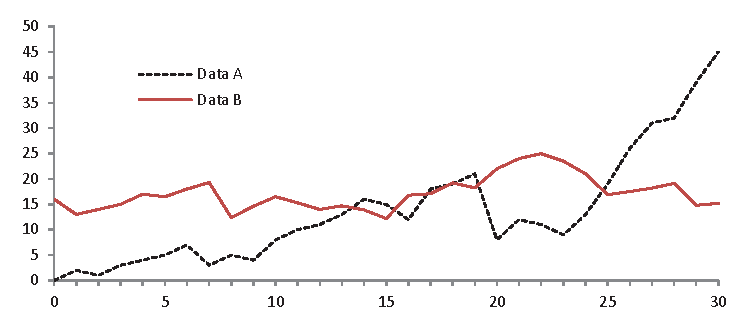
\includegraphics[width=\textwidth]{fig1.eps}
% \caption{A figure caption is always placed below the illustration.
% Please note that short captions are centered, while long ones are
% justified by the macro package automatically.} \label{fig1}
% \end{figure}



% ---- Bibliography ----
%
% BibTeX users should specify bibliography style 'splncs04'.
% References will then be sorted and formatted in the correct style.
%
\bibliographystyle{splncs04}
\bibliography{mybibliography}

Do check for citation formatting using Google Scholar
%
\end{document}
